\chapter{Introducción\label{sec:introduccion}}

Desde el principio de los tiempos la humanidad se ha esforzado por comprender el entorno que le rodea, aprender de él y usarlo en su propio beneficio para conseguir así hacer su vida más fácil. Por el momento hemos conseguido hacer volar aviones gracias a la observación de los pájaros o crear sistemas de sonar que se asemejan al sistema que utilizan los murciélagos para orientarse. Pero irónicamente, a pesar del esfuerzo invertido, nuestro propio cuerpo sigue albergando secretos que desentrañar que podrían facilitarle la vida a un gran número de personas.

El estudio del cuerpo humano ha sido uno de los temas más polémicos y que más ha evolucionado desde que hay registro. Aunque al comienzo estuvo muy marcado por la superstición y la religión, achacando la mayoría de las dolencias y efectos científicos a la magia, con el paso del tiempo aparecieron personas como Hipócrates y Aristóteles que fueron capaces de aportar un nuevo enfoque basado en la observación y estudio de lo que les rodeaba, asentando unas bases que, posteriormente, serían aprovechadas y mejoradas hasta convertirse en lo que conocemos hoy en día como método científico.

El estudio del cuerpo humano ha seguido diferentes fases a lo largo de la historia. Comparar el cuerpo humano con animales fue uno de los primeros pasos para descubrir cómo estábamos formados por dentro. Posteriormente, aprovechando los cuerpos de personas ya fallecidas se estudió la anatomía humana, permitiendo así crear mapas y dibujos de la estructura del cuerpo humano y sus órganos bastante detallados.

\begin{figure} [H]
    \centering
    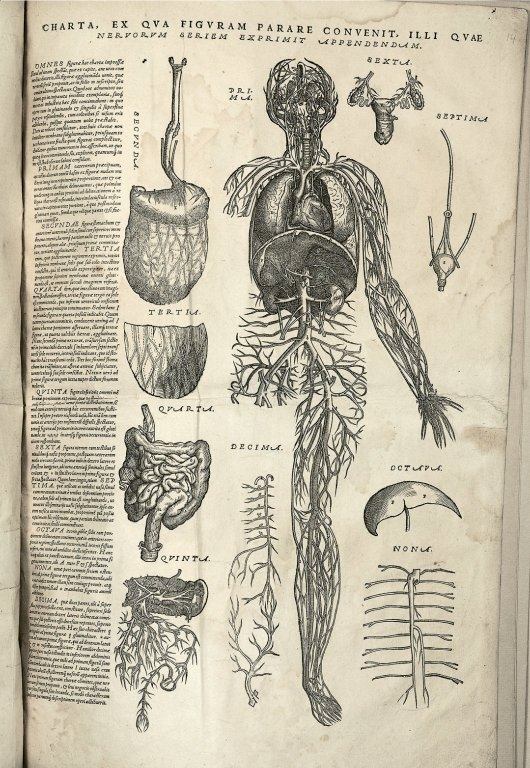
\includegraphics[width=0.25\textwidth]{Anatomia}
    \caption{Ejemplo de anatomía humana.}
    \label{fig:Anatomia}
\end{figure}

Pese a todo, estudiar cuerpos inertes tiene sus limitaciones de modo que durante un tiempo se realizaron vivisecciones para poder comprender mejor como funcionaban todos aquellos órganos, músculos y nervios que ya habían visto con anterioridad. Con el paso del tiempo este sistema fue descartado ya que es una práctica que ponía en peligro la vida del sujeto, haciéndolo pasar por una experiencia terrible en el mejor de los casos.

En la actualidad, gracias al conocimiento acumulado de muchos años y a los avances en otros campos de la ciencia, se han desarrollado dispositivos y técnicas que permiten el estudio en vivo del comportamiento del cuerpo humano de forma no invasiva. Es posible utilizar ecografías para ver el estado del corazón, radiografías para diagnosticar un hueso roto e incluso técnicas más avanzadas como la medicina nuclear que permiten saber que partes del cerebro se activan frente a determinados estímulos sin necesidad de interactuar físicamente con él.

Si bien todas las técnicas anteriores han supuesto auténticos hitos en la medicina moderna y han permitido diagnosticar un gran número de enfermedades así como mejorar la calidad de vida de muchas personas, la mayoría presenta inconvenientes que hacen improbable su uso a nivel personal o docente debido al tamaño de los equipos necesarios para su realización o el coste muy elevado del procedimiento (sin contar con el conocimiento necesario para la realización correcta de la prueba).

Teniendo en mente esta problemática se han desarrollado dispositivos capaces de medir pequeñas las variaciones de voltaje que se producen en el interior de nuestro cuerpo haciendo uso de unos dispositivos denominados electrodos.
\\De esta forma es posible, con un coste muy reducido y un equipamiento relativamente asequible, conseguir inferir que procesos químicos y físicos se están produciendo en el interior de nuestro cuerpo.

Haciendo uso de este sistema y en función del origen de dichas señales dichos registros reciben distintos nombres: electrocardiograma (ECG) para las señales originadas por las contracciones del corazón; electromiograma (EMG) para las generadas en los músculos; electroencefalograma (EEG) para aquellas generadas en el cerebro, etc.

\begin{figure} [H] %this figure will be at the center
    \centering
    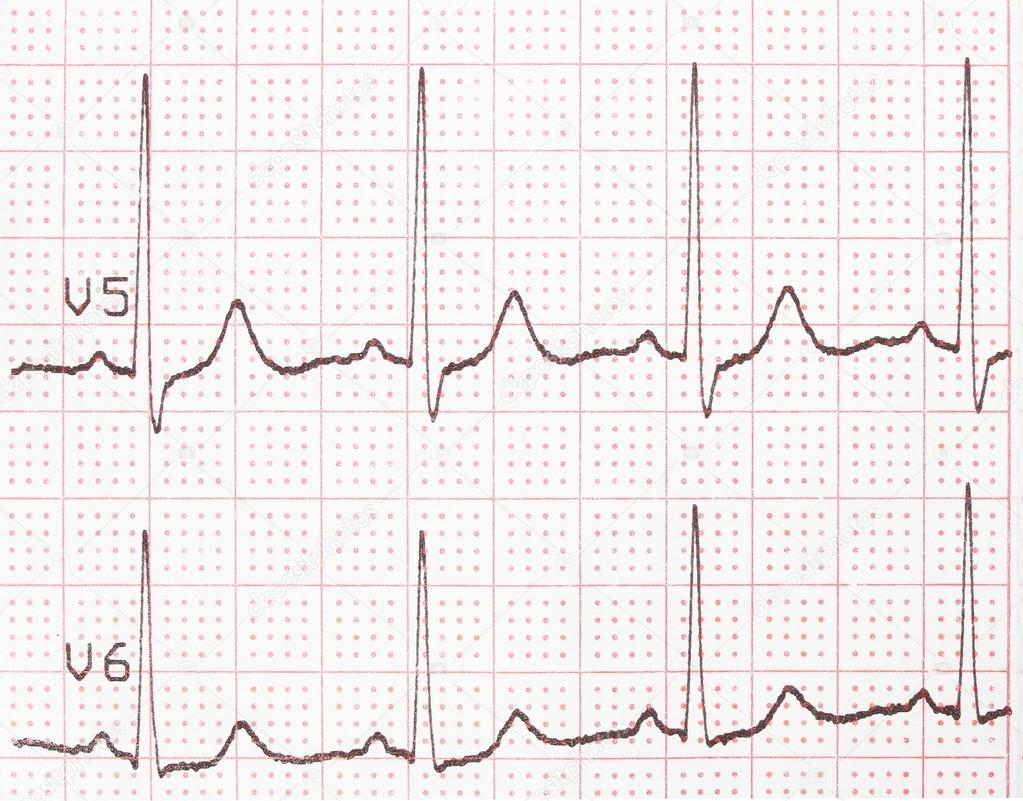
\includegraphics[width=10cm]{ECG}
    \caption{Ejemplo de ECG}
    \label{fig:ECG}
\end{figure}

\section{Alcance y estructura del proyecto}
El objetivo de este proyecto es realizar un sistema capaz de captar señales de electroencefalogramas (EEG) manteniendo una buena relación prestaciones/coste. El sistema estará compuesto de dos tarjetas, una de acondicionamiento y de adquisición de datos basada en el circuito integrado ADS1299 y otra de procesamiento y transmisión de dicha información. Esta última es el objetivo del presente proyecto. La plataforma de procesamiento estará basada en un procesador de altas prestaciones, dispondrá de interfaces Wifi, Bluetooth y almacenamiento USB para la transmisión y almacenamiento de los datos respectivamente. 

En la primera fase del proyecto se seleccionará el microcontrolador más adecuado entre los existentes en el mercado analizando características como: capacidad de procesado, interoperación con otros dispositivos, prestaciones...
\\Se compararán los microcontroladores ofrecidos por los distintos fabricantes (ST Microelectronics, Texas instruments, etc) y finalmente, se escogerá aquel que mejor se adecúe a las necesidades del proyecto siendo los principales candidatos los de la familia ARM-M4 STM32F4x por su excelente relación prestaciones-coste.
\\Se valorará también la posibilidad de utilizar diferentes herramientas para la programación del microcontrolador y las alternativas open source en caso de existir.

Una vez hecho el diseño eléctrico de la tarjeta se procederá al diseño de una PCB, la cual se implementará utilizando tecnología SMD en su mayor parte. Para el diseño de la placa se utilizará KiCad por las numerosas ventajas que presenta al ser software libre y la gran cantidad de información que se puede encontrar sobre el funcionamiento del mismo.
Tras depurar la PCB, se implementará un sencillo firmware que permita testear el hardware diseñado y hacer una adquisición básica utilizando la tarjeta SAD utilizando los distintos interfaces implementados.

Adicionalmente se pondrá en marcha un programa para el ordenador basado en LabView donde presentar los datos recibidos.

\section{Base teórica\label{sec:Base_teorica}}

% Documentación interesante para esta sección: 
% http://slideplayer.es/slide/3413933/

Antes de empezar a desarrollar el dispositivo ya mencionado es indispensable realizar una investigación previa que debe abarcar desde el origen de las señales que se quieren adquirir hasta el 

Partes a redactar de esta sección:
\begin{itemize}
\item base física/química de las señales del cerebro
\item tipos de señales:
\begin{itemize}
	\item características físicas de las señales
	\item información asociada a cada tipo
\end{itemize}
\item posiciones donde se pueden medir
\end{itemize}